\newpage

\appendix \addcontentsline{toc}{section}{Appendix}

    \section{Appendix A: Schematics} \label{appendix:schematics}

        \begin{figure}[ht]
            \begin{center}
                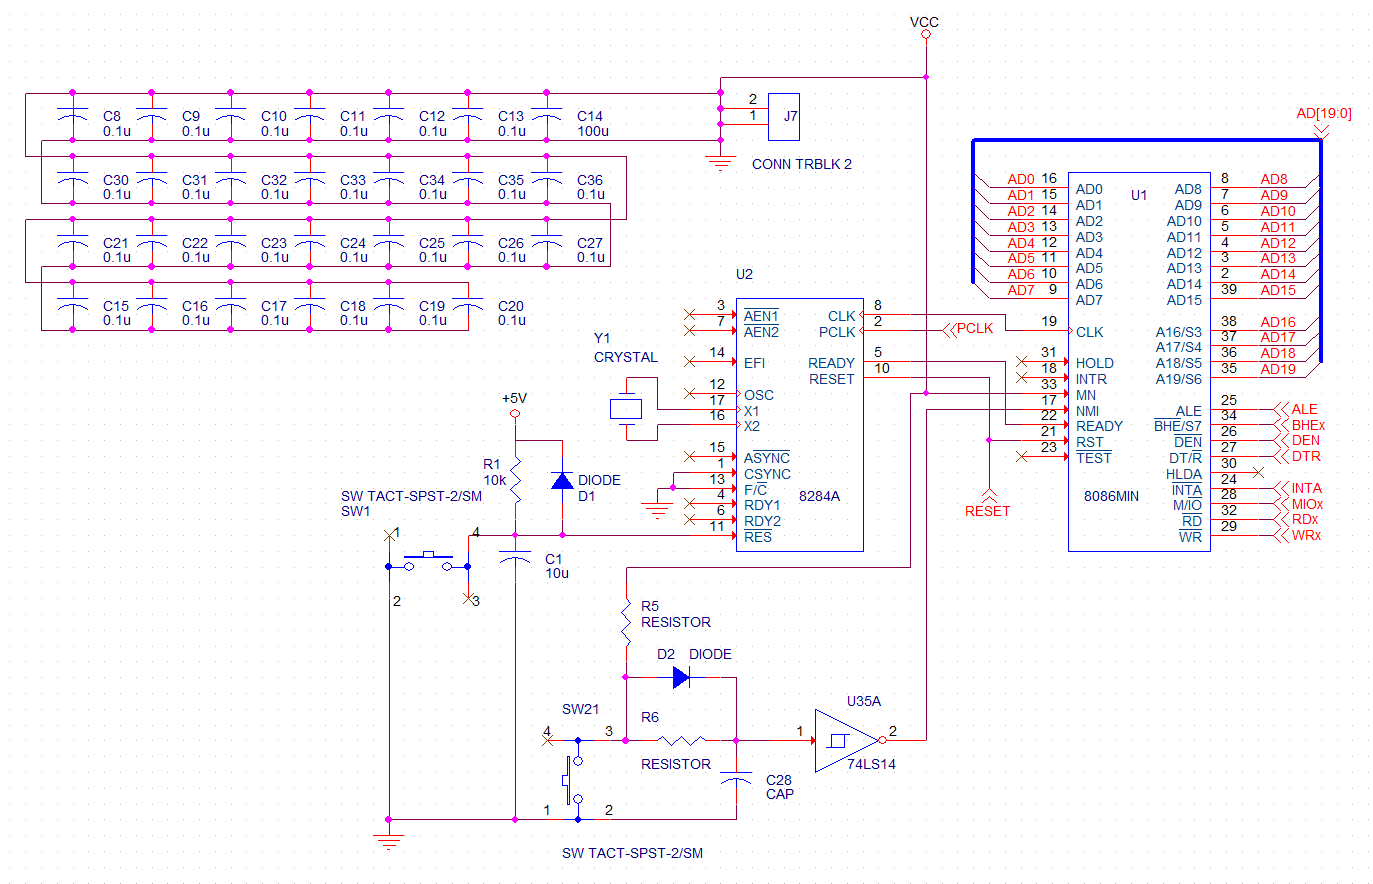
\includegraphics[width=1\textwidth]{figures/schematics/8086.png}
                \caption{8086 interfaced with the 8284A clock generator and its Reset RC Push Button Circuit, and the Power Bank of the Board} \label{fig:page1}
            \end{center}
        \end{figure}

        \begin{figure}[ht]
            \begin{center}
                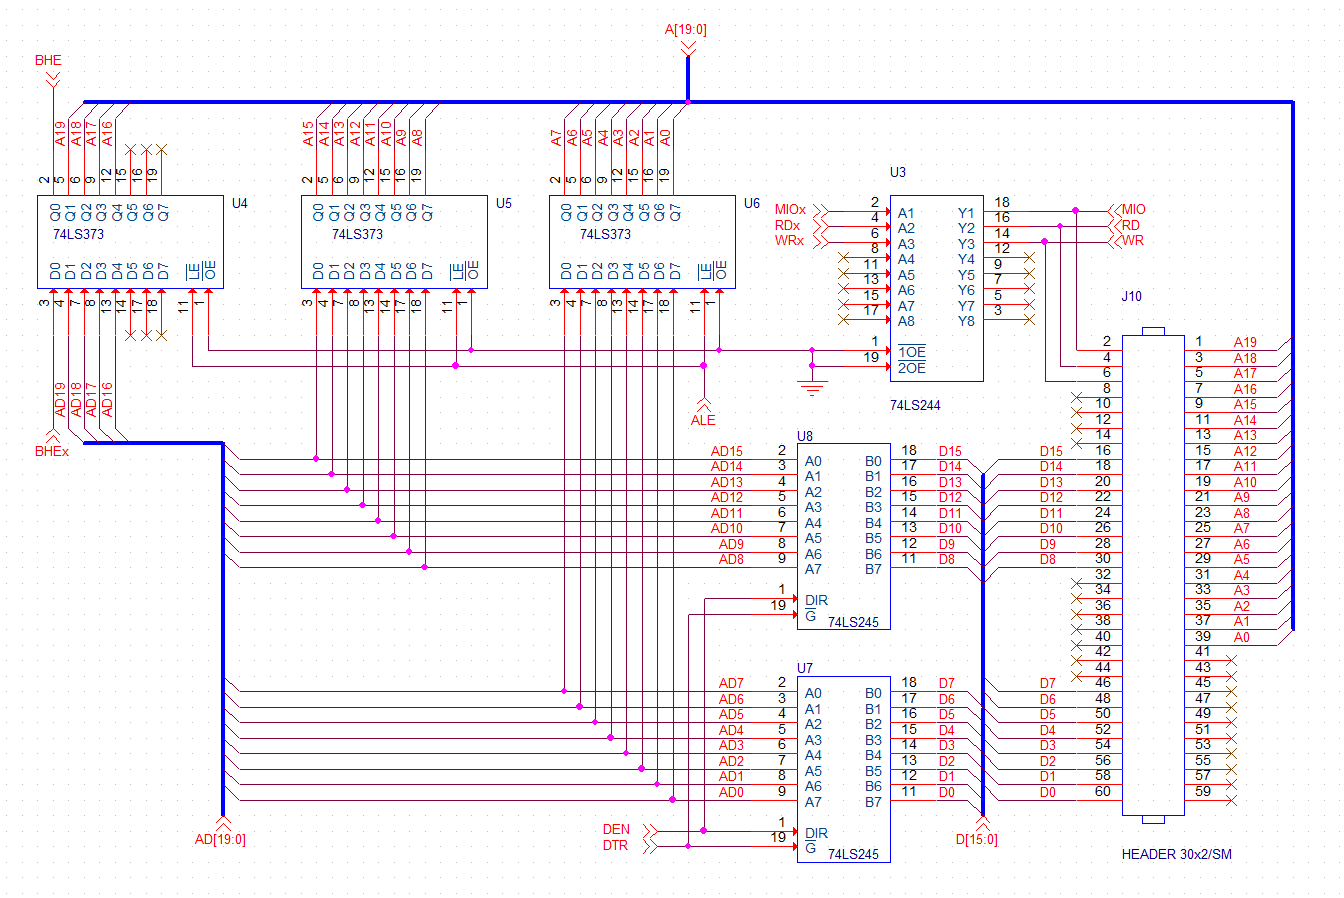
\includegraphics[width=1\textwidth]{figures/schematics/buffers.png}
                \caption{8086 Demultiplexed with Address and Data Buses Pulled into Headers} \label{fig:page2}
            \end{center}
        \end{figure}

        \begin{figure}[ht]
            \begin{center}
                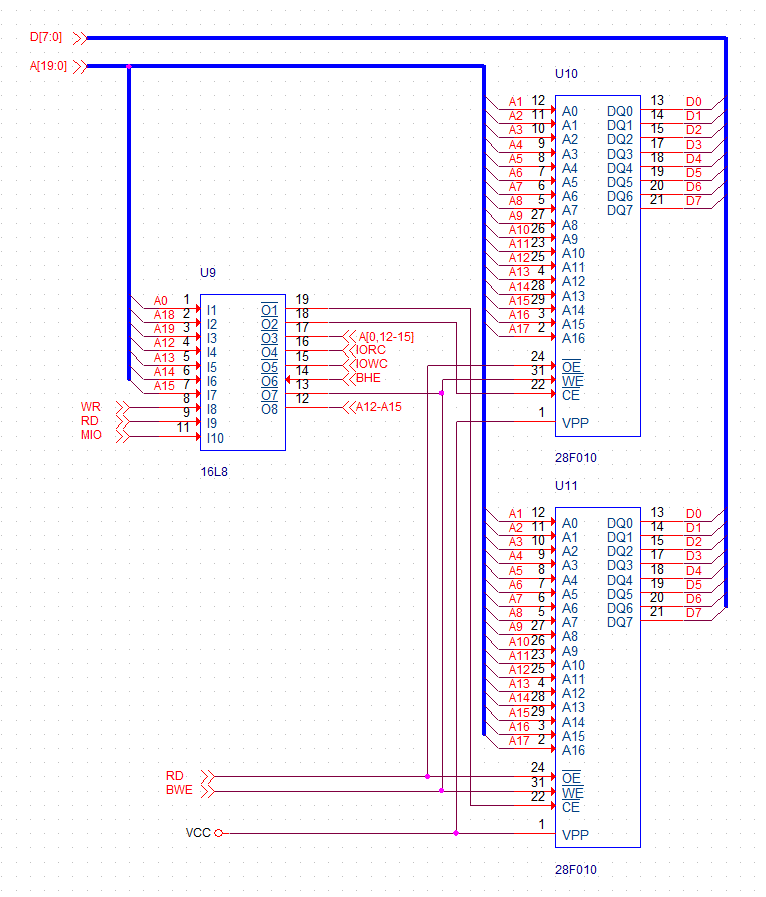
\includegraphics[width=1\textwidth]{figures/schematics/flash_mem.png}
                \caption{256 kB of CMOS Flash Memory and 128 kB Static SRAM} \label{fig:page3}
            \end{center}
        \end{figure}

        \begin{figure}[ht]
            \begin{center}
                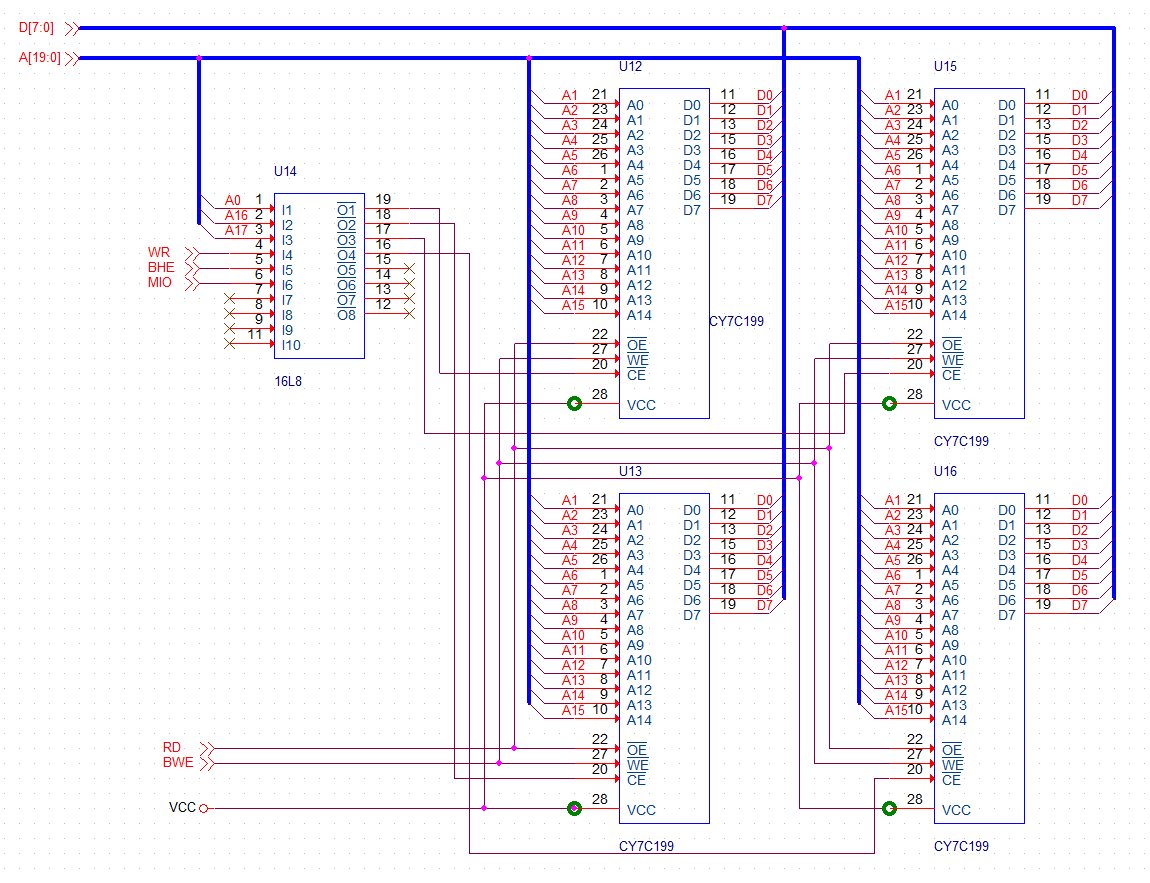
\includegraphics[width=1\textwidth]{figures/schematics/sram.png}
                \caption{128 kB Static SRAM} \label{fig:page4}
            \end{center}
        \end{figure}

        \begin{figure}[ht]
            \begin{center}
                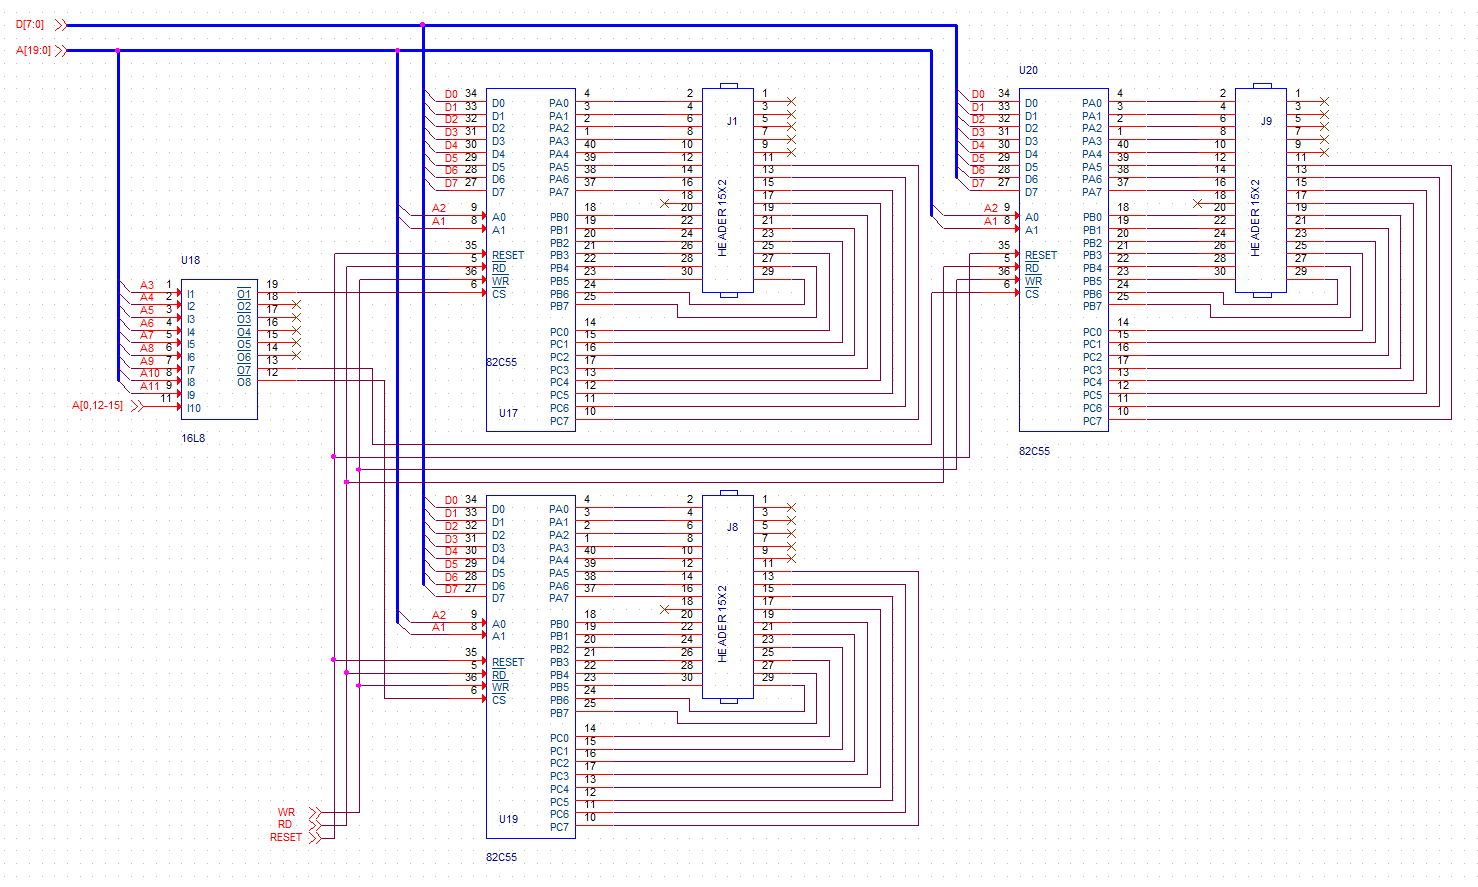
\includegraphics[width=1\textwidth]{figures/schematics/ppi.png}
                \caption{Programmable Peripheral Interface Chips with Port Connections Pulled into Headers} \label{fig:page5}
            \end{center}
        \end{figure}

        \begin{figure}[ht]
            \begin{center}
                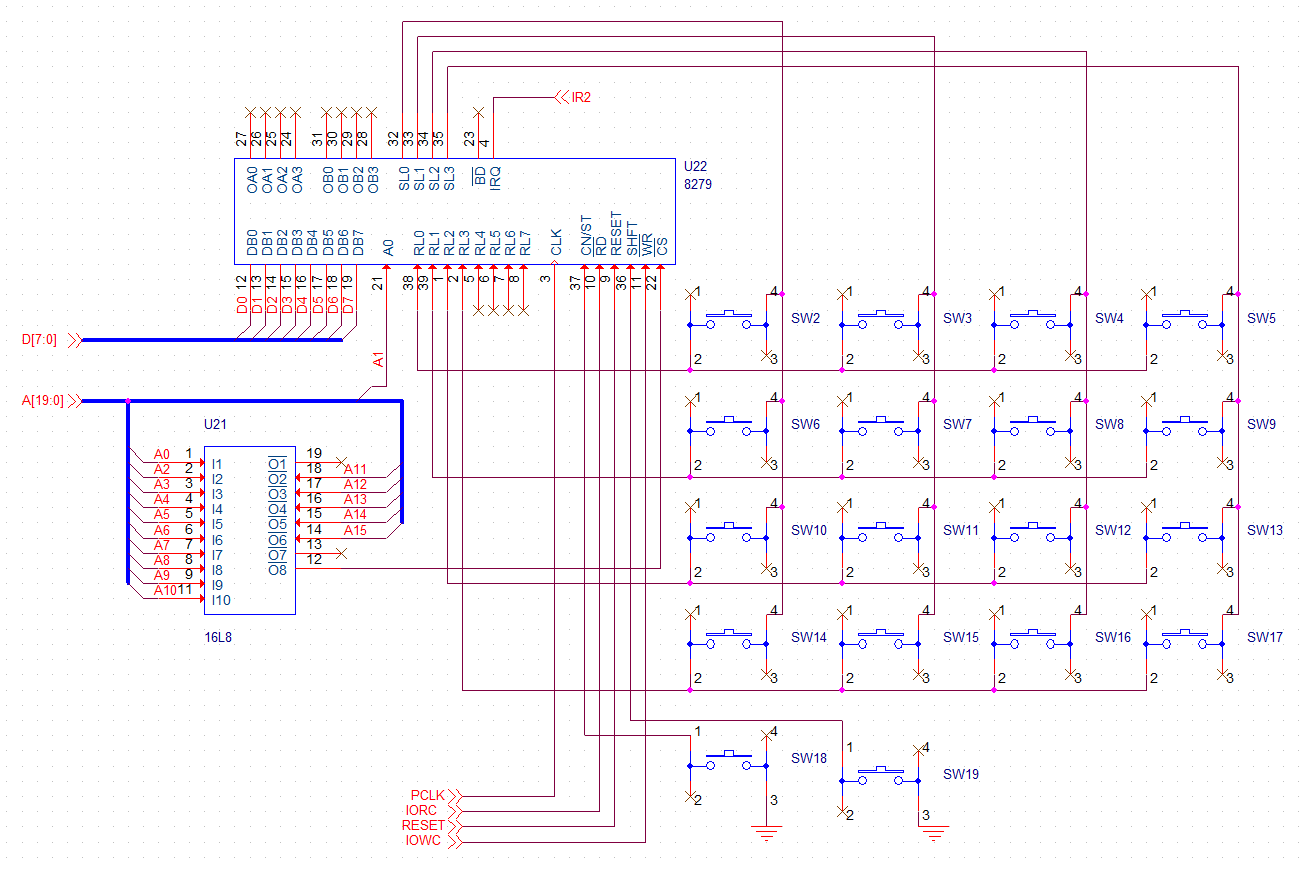
\includegraphics[width=1\textwidth]{figures/schematics/keyboard.png}
                \caption{5$\times$4 Keyboard Matrix} \label{fig:page6}
            \end{center}
        \end{figure}

        \begin{figure}[ht]
            \begin{center}
                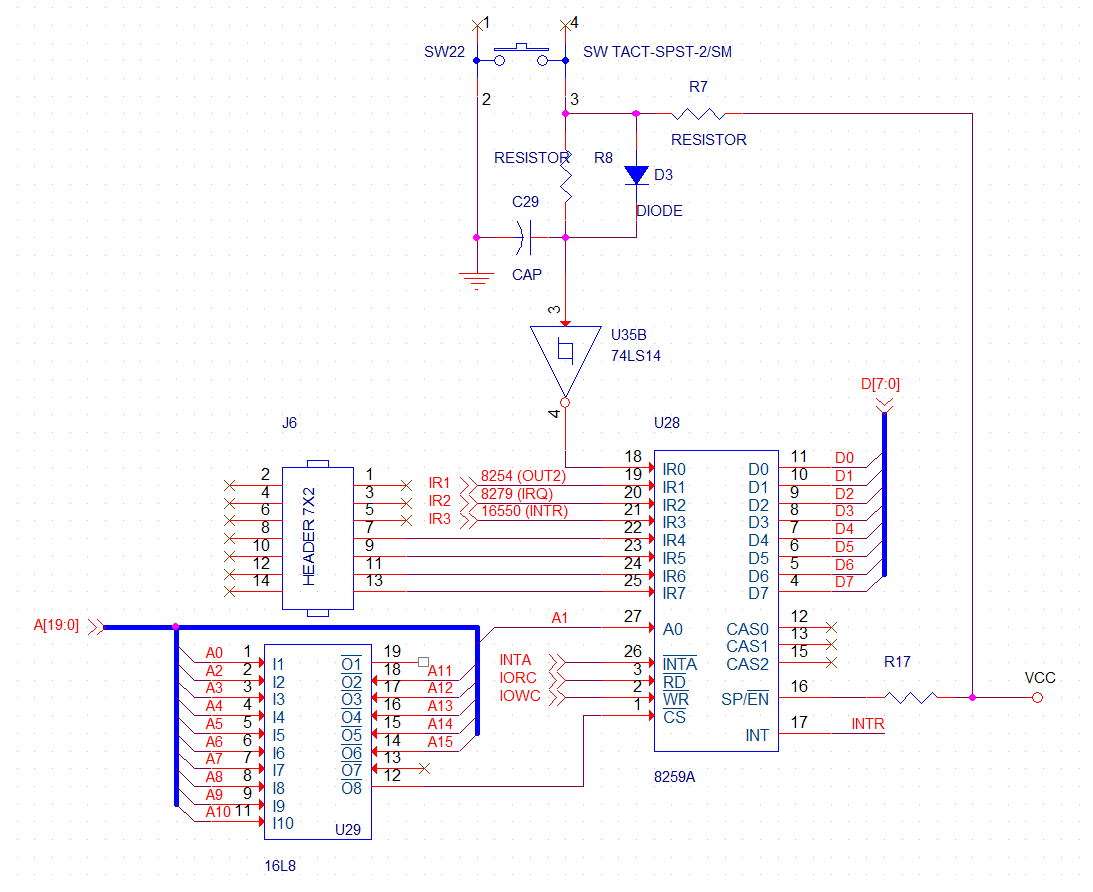
\includegraphics[width=1\textwidth]{figures/schematics/pic.png}
                \caption{Programmable Interval Timer} \label{fig:page7}
            \end{center}
        \end{figure}

        \begin{figure}[ht]
            \begin{center}
                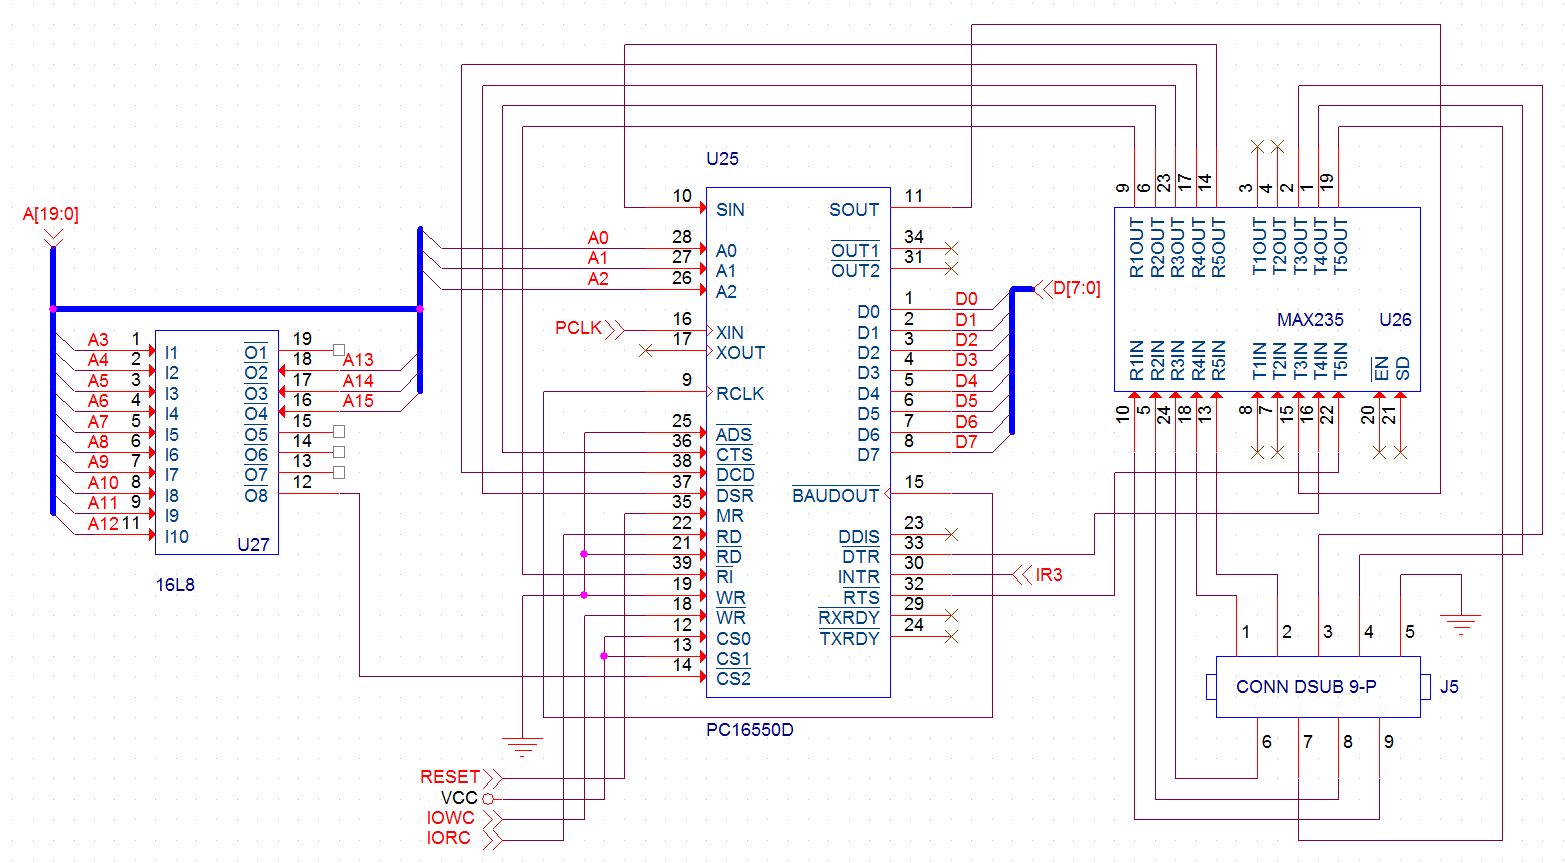
\includegraphics[width=1\textwidth]{figures/schematics/uart.png}
                \caption{UART Connected for Serial Port Using a Line Driver/Receiver and a DSUB-9 connector} \label{fig:page8}
            \end{center}
        \end{figure}

        \begin{figure}[ht]
            \begin{center}
                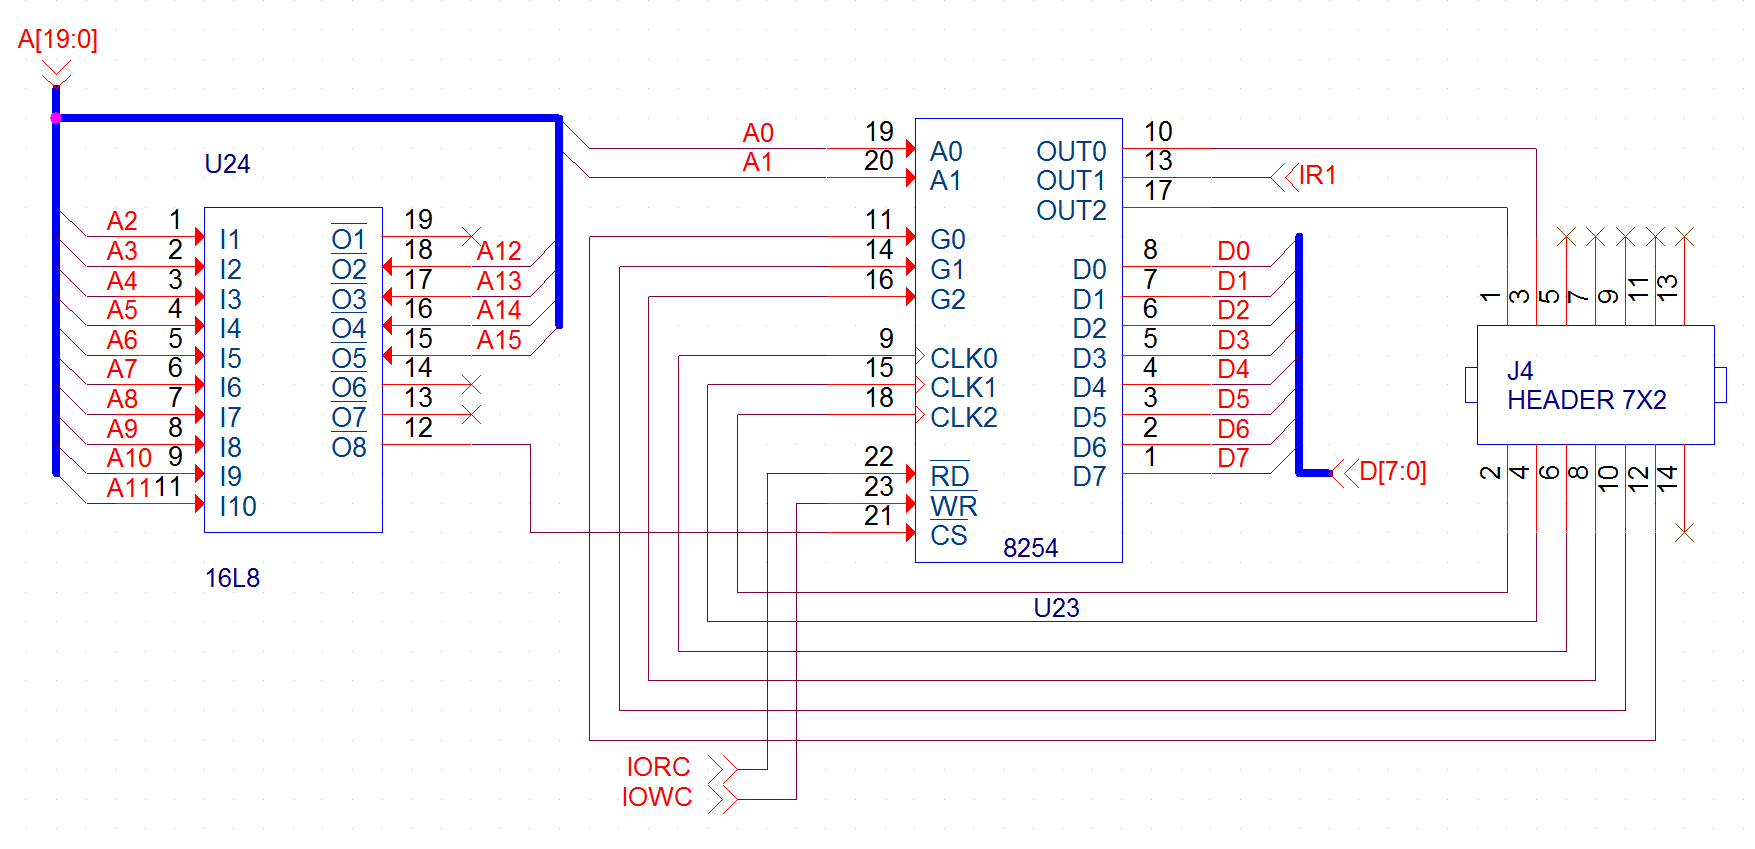
\includegraphics[width=1\textwidth]{figures/schematics/pit.png}
                \caption{Programmable Interrupt Controller with Headers fro External Access} \label{fig:page9}
            \end{center}
        \end{figure}

        \begin{figure}[ht]
            \begin{center}
                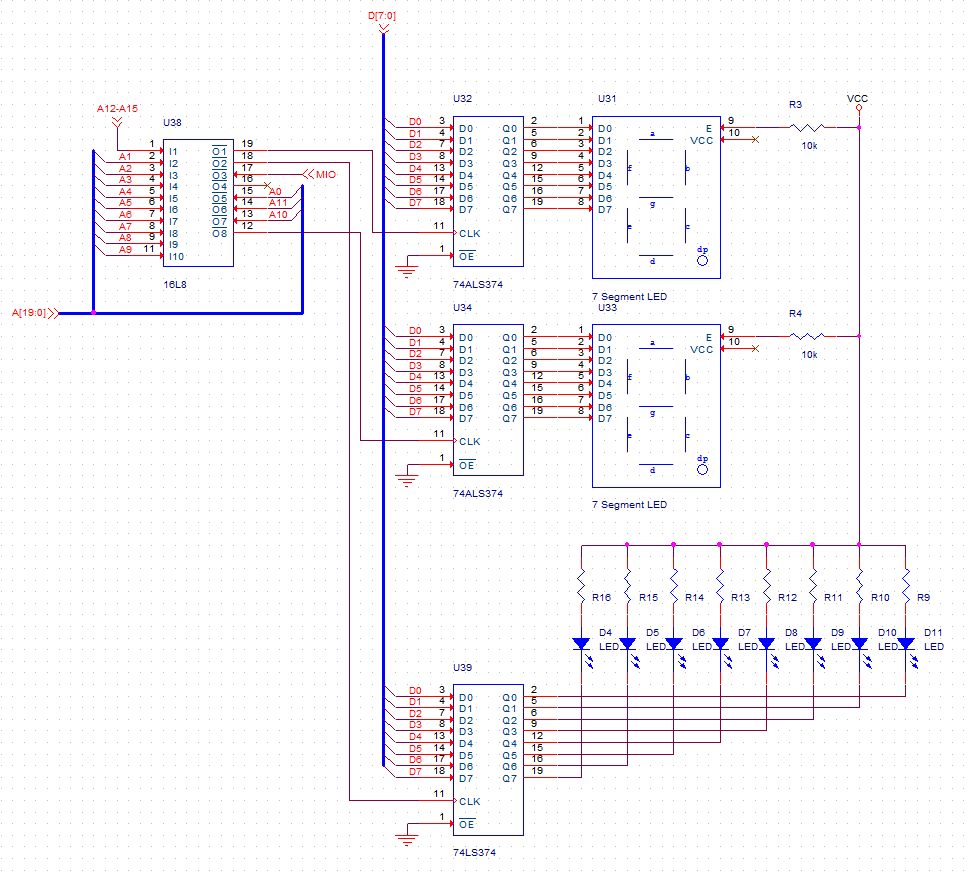
\includegraphics[width=1\textwidth]{figures/schematics/led.png}
                \caption{Common-Anode 7-Segment LEDs with 8 LEDs} \label{fig:page10}
            \end{center}
        \end{figure}

        \begin{figure}[ht]
            \begin{center}
                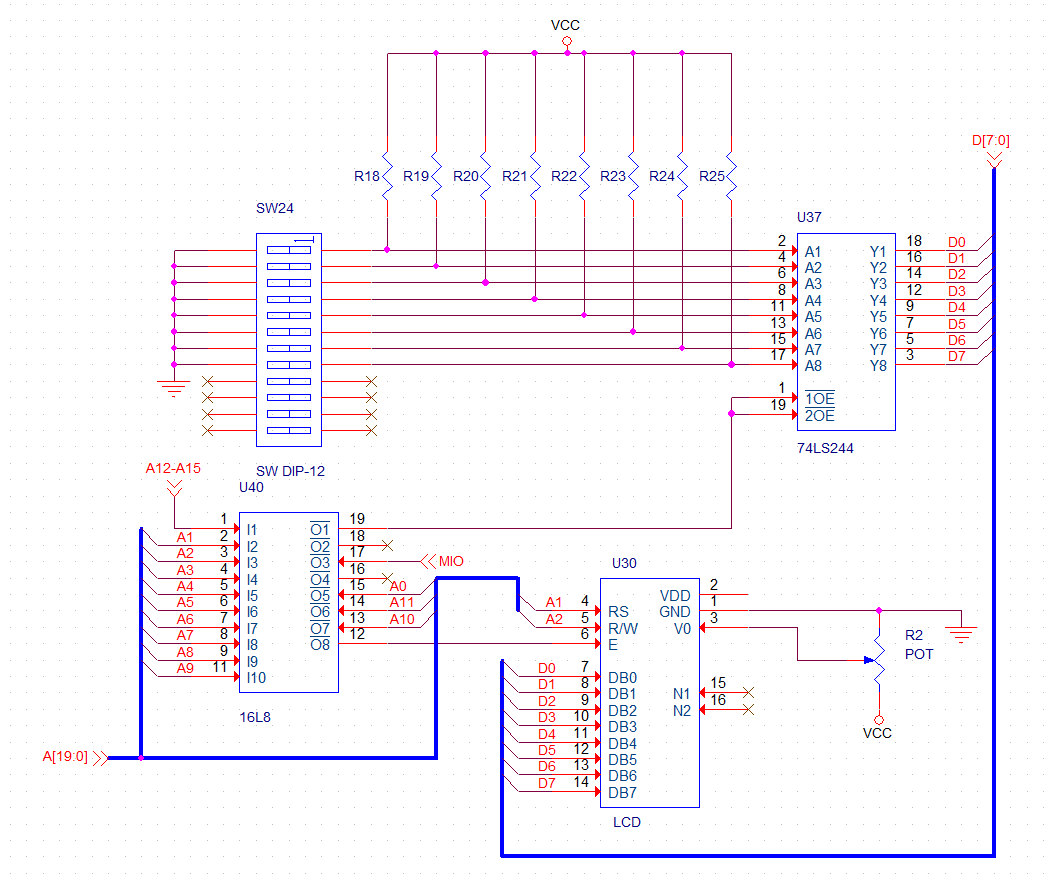
\includegraphics[width=1\textwidth]{figures/schematics/lcd.png}
                \caption{20 character $\times$ 4 line LCD Display with an Integrated LCD Controller} \label{fig:page11}
            \end{center}
        \end{figure}


    \clearpage
    \newpage

    \section{Appendix B: Code Implementations} \label{appendix:code}

        \subsection{Programmable Logic Devices}

            \subsubsection{U9}

                \VerbatimInput{hdl/u09.vhd}

            \newpage
            \subsubsection{U14}

                \VerbatimInput{hdl/u14.vhd}

            \newpage
            \subsubsection{U18}

                \VerbatimInput{hdl/u18.vhd}

            \newpage
            \subsubsection{U21}

                \VerbatimInput{hdl/u21.vhd}

            \newpage
            \subsubsection{U24}

                \VerbatimInput{hdl/u24.vhd}

            \newpage
            \subsubsection{U27}

                \VerbatimInput{hdl/u27.vhd}

            \newpage
            \subsubsection{U29}

                \VerbatimInput{hdl/u29.vhd}

            \newpage
            \subsubsection{U38}

                \VerbatimInput{hdl/u38.vhd}

            \newpage
            \subsubsection{U40}

                \VerbatimInput{hdl/u40.vhd}

        \newpage
        \subsection{Assembly Implementations}

            \subsubsection{LCD} \label{sec:lcd_asm}
                \VerbatimInput{assembly/lcd.asm}

            \newpage
            \subsubsection{Keyboard} \label{sec:keybrd_asm}
                \VerbatimInput{assembly/keyboard.asm}


    \clearpage
    \newpage

    \section{Appendix C: PCB Layouts} \label{appendix:pcb}

        \begin{figure}[ht]
            \begin{center}
                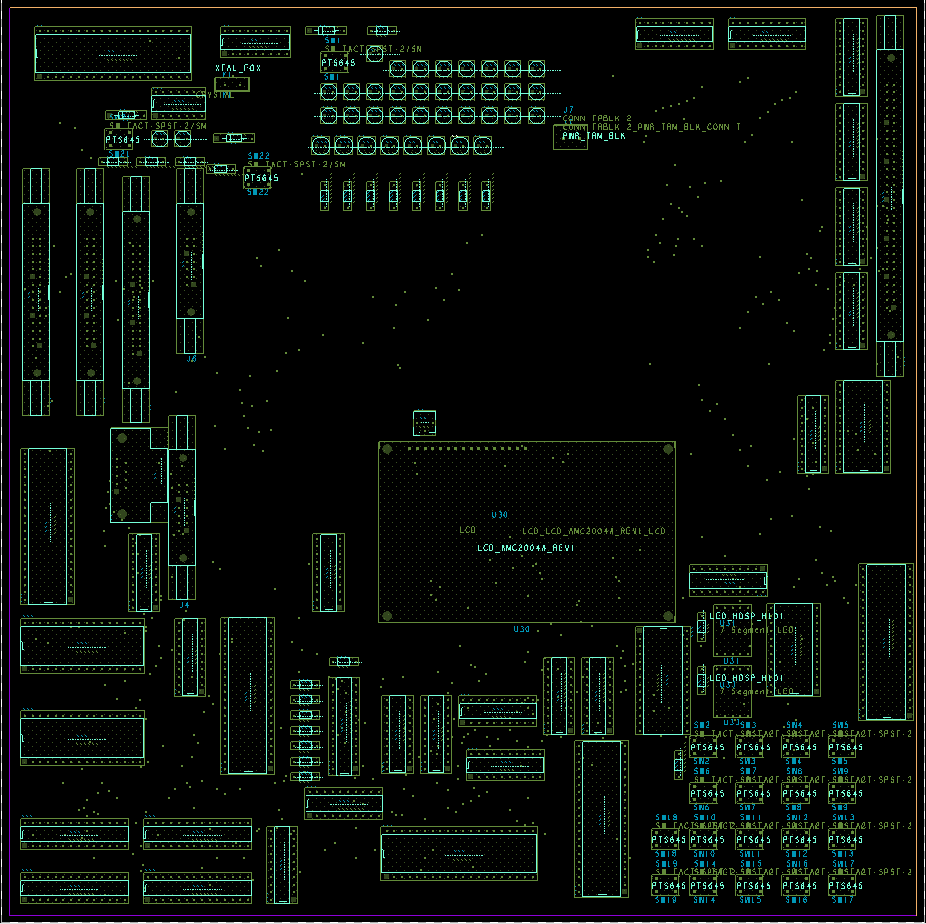
\includegraphics[width=0.9\textwidth]{figures/main.png}
                \caption{8086 interfaced with the 8284A clock generator and its Reset RC Push Button Circuit, and the Power Bank of the Board} \label{fig:main}
            \end{center}
        \end{figure}

        \begin{figure}[ht]
            \begin{center}
                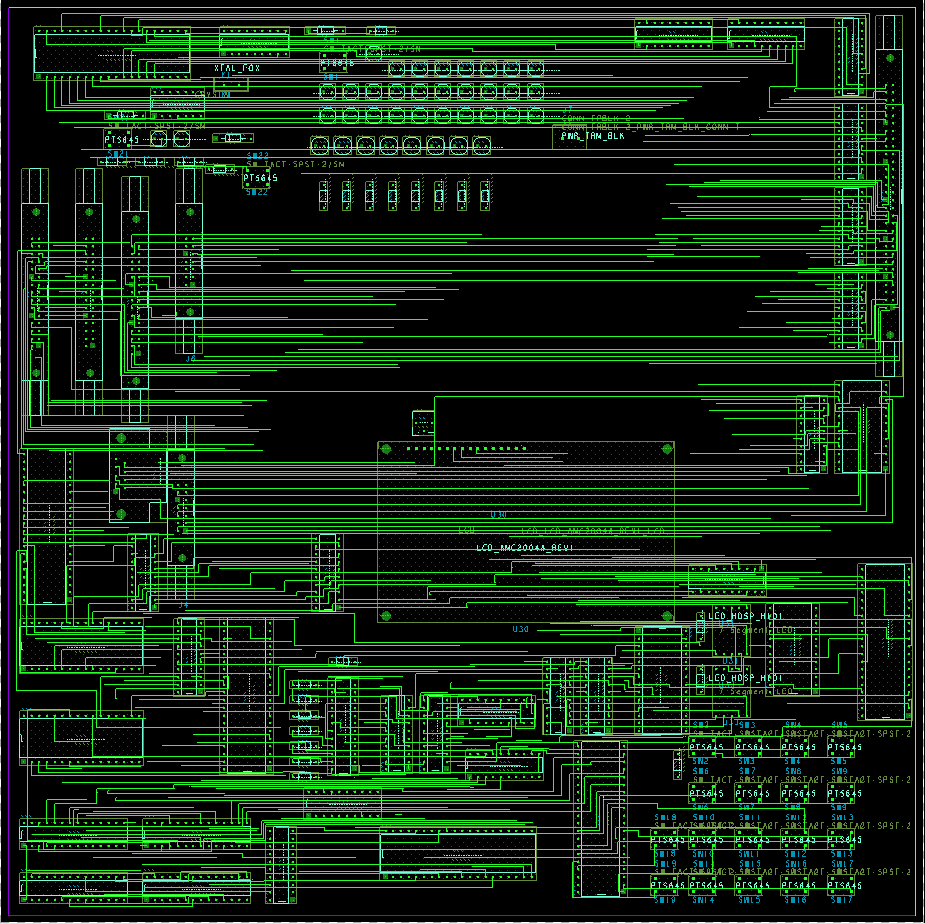
\includegraphics[width=0.95\textwidth]{figures/top.png}
                \caption{8086 interfaced with the 8284A clock generator and its Reset RC Push Button Circuit, and the Power Bank of the Board} \label{fig:top}
            \end{center}
        \end{figure}

        \begin{figure}[ht]
            \begin{center}
                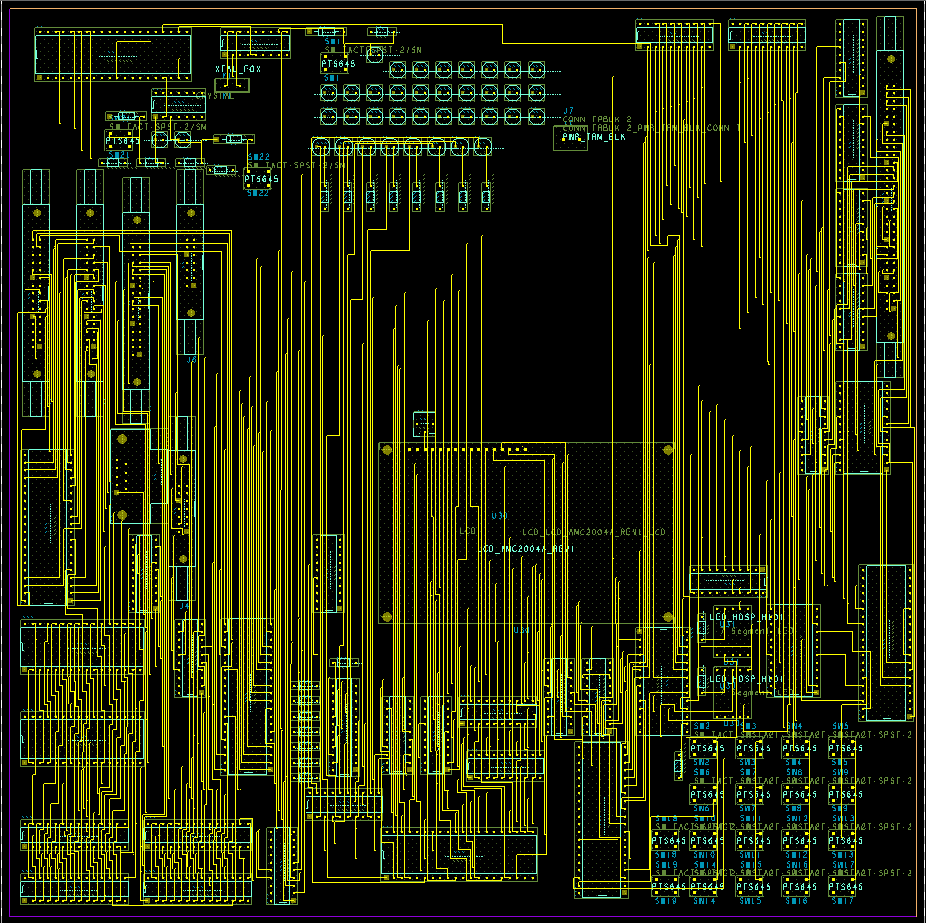
\includegraphics[width=0.95\textwidth]{figures/bottom.png}
                \caption{8086 interfaced with the 8284A clock generator and its Reset RC Push Button Circuit, and the Power Bank of the Board} \label{fig:bottom}
            \end{center}
        \end{figure}

        \begin{figure}[ht]
            \begin{center}
                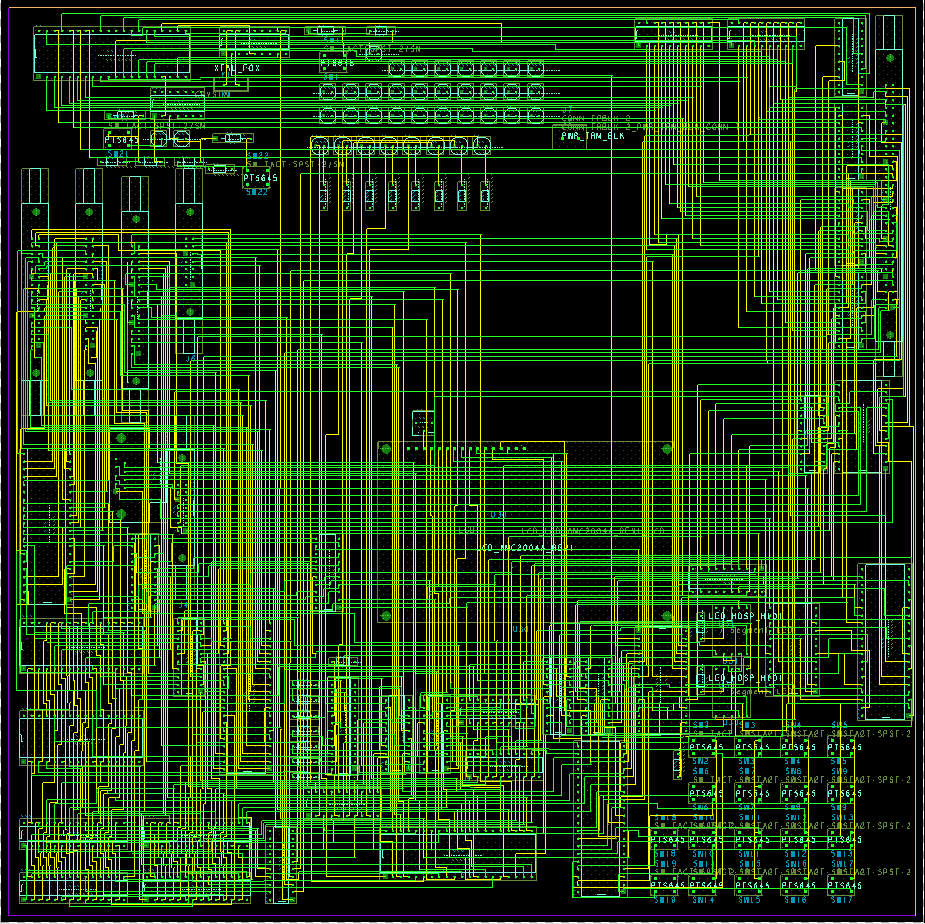
\includegraphics[width=0.95\textwidth]{figures/board.png}
                \caption{8086 interfaced with the 8284A clock generator and its Reset RC Push Button Circuit, and the Power Bank of the Board} \label{fig:board}
            \end{center}
        \end{figure}

        \begin{figure}[ht]
            \begin{center}
                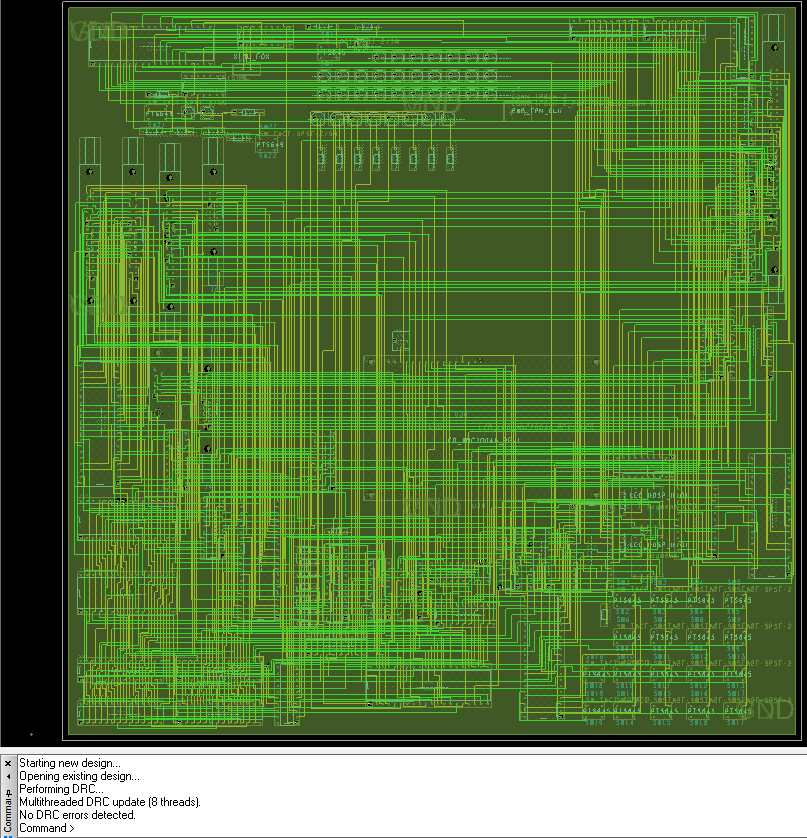
\includegraphics[width=0.95\textwidth]{figures/all.png}
                \caption{8086 interfaced with the 8284A clock generator and its Reset RC Push Button Circuit, and the Power Bank of the Board} \label{fig:all}
            \end{center}
        \end{figure}

        \clearpage
